% Provenance (never printed): see sources/outline_sources.md (Year 2: palaeogeography through
% the Phanerozoic; sea level; orogenies; mass extinctions and their Earth causes). Maps from the
% plate model of Merdith and others (2021) through the GPlates Web Service; sea level from the
% Miller and others (2005) NOAA study (Haq and others 1987; Kominz and others 2008); flooding and
% the Pitman model after Tasistro-Hart and Macdonald (2023); the big five after Marshall (2023)
% and Kaiho (2022); oceanic anoxic events after Rigo and others (2024) and Walker-Trivett and
% others (2024); CAMP carbon dioxide after Capriolo and others (2020); Chicxulub after
% Pickersgill and others (2026) and Collins and others (2020). Curves and numbers from
% figdata/bachelor-2/phanerozoic.py; exercise and problem values in the Book 4 scratch
% calculator calc/ch19.py.
\chapter{La Tierra fanerozoica}\label{ch:b2:phanerozoic-earth}

En el oeste de Kansas, en pleno centro de Norteamérica, se alzan sobre la pradera pilares de creta blanca.
La creta es el fango de un fondo marino: hace unos 80 millones de años, un
mar somero cruzaba de norte a sur el centro de Norteamérica, y los caparazones de
algas flotantes se depositaban en su fondo a unas centésimas de milímetro al año. Cinco veces en los
últimos 540 millones de años, una gran parte de las especies que vivían en mares así desapareció en un
instante geológico. Ambas historias son propias de la Tierra: los continentes se movieron y el mar subió y bajó sobre
ellos, y al menos tres de las cinco grandes extinciones coincidieron con efusiones de lava procedentes del interior
del planeta. Este capítulo recorre el Fanerozoico a través de sus mapas, su nivel del mar, sus cordilleras
y sus crisis, y pone cifras a dos de ellos: cuánto hacen subir el mar las dorsales y cuánta
tierra ahoga un mar más alto.
% ledger: kgs:monument-rocks, kgs:chalk, ics:base.Phanerozoic, kaiho22:table, cr03:table

\begin{recall}
\textbf{De los volúmenes escolares}: la tectónica de placas y Pangea; los fósiles y la escala de tiempo
geológico; las transgresiones leídas en un acantilado. \textbf{Del volumen de primer año}: la ley profundidad--edad del
fondo oceánico; la curva hipsométrica; la isostasia; la eustasia y el nivel relativo del mar; las grandes
provincias ígneas; las extinciones masivas como marcadores estratigráficos, el iridio del límite K--Pg y la
datación de la crisis del final del Pérmico; los pisos y los GSSP. \textbf{De capítulos anteriores}: los \omterm{def:b2:alpine-orogen:orogen}{orógenos}
(\cref{ch:b2:alpine-orogen,ch:b2:himalaya-andes}); el \omterm{def:b2:wilson-cycle:wilson}{ciclo de Wilson} y los \omterm{def:b2:wilson-cycle:supercontinent}{supercontinentes}
(\cref{ch:b2:wilson-cycle}); el \omterm{def:b2:basins-compared:backstripping}{backstripping} (\cref{ch:b2:basins-compared}); las bolas de nieve del
Criogénico (\cref{ch:b2:precambrian-earth}). La extinción y la historia de la vida corresponden a los
libros de biología; el volumen de tercer año trata el paleomagnetismo y la estratigrafía secuencial.
\end{recall}

\section{Mapas de un mundo en movimiento}\label{sec:b2:phanerozoic-earth:maps}

Una roca rara vez está donde se formó. Un carbón, una arenisca de desierto, un arrecife: cada uno se depositó a
cierta latitud y ha sido transportado desde entonces por su placa. Antes de poder leer en esas rocas el clima o la vida de
una época pasada, hay que devolverlas al lugar donde estaban.

\begin{definition}[Paleogeografía; mapa paleogeográfico]\label{def:b2:phanerozoic-earth:palaeogeography}
La \emph{paleogeografía}\index{paleogeografia@paleogeografía} es la reconstrucción de la geografía de una época
pasada: las posiciones de los continentes y los océanos, y de sus líneas de costa, cordilleras y
mares. Un \emph{mapa paleogeográfico}\index{mapa paleogeografico@mapa paleogeográfico} muestra esa geografía en un
momento dado, sobre la cuadrícula de latitud y longitud de ese momento.
\end{definition}

Cuatro clases de pruebas entran en un mapa así. La imanación de las rocas da la latitud a la
que se formaron, objeto del paleomagnetismo en el volumen de tercer año; pero el campo terrestre es
simétrico respecto de su eje, así que no dice nada de la longitud. El fondo oceánico registra directamente el movimiento de
las placas, a través de sus bandas magnéticas y sus edades, pero solo hasta el
fondo superviviente más antiguo, de unos 190 millones de años: todo lo anterior ha sido subducido. Antes de eso,
el encaje de los continentes, las suturas y los \omterm{def:b2:alpine-orogen:orogen}{orógenos} donde se cerraron océanos, y los fósiles y
sedimentos que delatan un clima ---arrecifes y evaporitas en los trópicos, depósitos glaciares cerca de los
polos--- completan el cuadro. Los modelos de placas reúnen estas restricciones y hacen retroceder cada placa en el
tiempo; las reconstrucciones deben tener en cuenta además la lenta rotación de toda la Tierra sólida respecto
de su eje de giro, llamada deriva polar verdadera.
% ledger: vh26:palaeogeography, gws:merdith-frame, data:b2-seafloor-age, merdith21:model

\begin{omfigure}
\centering
% figdata/bachelor-2/phanerozoic.py parts map-<t>, cities-<t>, grat (Mollweide, x and y in Earth radii)
\begin{tikzpicture}
\begin{groupplot}[group style={group size=2 by 3, horizontal sep=0.35cm, vertical sep=0.55cm},
  width=0.53\linewidth, axis equal image, hide axis, clip=false,
  xmin=-2.85, xmax=2.85, ymin=-1.43, ymax=1.43,
  title style={font=\small, yshift=-1.5ex}]
\pgfplotsinvokeforeach{500,300,200,100,50,0}{
\nextgroupplot[title={#1~\unit{Ma}}]
\fill[omSea] (axis cs:0,0) ellipse [x radius=2.8284, y radius=1.4142];
\addplot[fill=omLithAlluv!85!black, draw=none] table[x=x, y=y]
  {figdata/out/bachelor-2-phanerozoic-map-#1.dat};
\addplot[black!35, line width=0.2pt] table[x=x, y=y] {figdata/out/bachelor-2-phanerozoic-grat.dat};
\draw[black!70, line width=0.4pt] (axis cs:0,0) ellipse [x radius=2.8284, y radius=1.4142];
\addplot[only marks, mark=*, mark size=1.3pt, red!75!black, point meta=explicit symbolic,
  nodes near coords, nodes near coords style={font=\tiny\bfseries, anchor=south west,
  inner sep=0.5pt, text=red!60!black}]
  table[x=x, y=y, meta=tag] {figdata/out/bachelor-2-phanerozoic-cities-#1.dat};
}
\end{groupplot}
\end{tikzpicture}
\par\smallskip{\small Las costas actuales llevadas a seis momentos del pasado en el modelo de placas de
Merdith y otros (2021), reconstruidas por el GPlates Web Service, en una proyección de Mollweide de áreas
iguales; paralelos cada \ang{30}, meridianos cada \ang{60}. Los puntos rojos siguen cuatro
ciudades: París (P), Nueva York (N), Sídney (S) y Ciudad del Cabo (C); a \qty{500}{Ma} la corteza de
Sídney todavía no está en el modelo. Las formas son las costas actuales desplazadas, no las costas de
aquellas épocas, y en este marco paleomagnético las longitudes son arbitrarias.}
\end{omfigure}
% ledger: data:b4-palaeocoast, data:b4-palaeopos, geonames4:cities, gws:merdith-frame, merdith21:model

Los seis mapas anteriores resumen el Fanerozoico. A \qty{500}{Ma} los continentes meridionales forman
una sola masa, Gondwana, buena parte de ella cerca del polo Sur, con la corteza de París a \ang{61}~S en su
margen. Hacia \qty{300}{Ma} los continentes se han unido en Pangea, ensamblada desde unos
\qty{325}{Ma} y fragmentada desde unos \qty{200}{Ma}: París y Nueva York están en el ecuador, Ciudad del
Cabo y Sídney cerca de \ang{60}~S. A \qty{200}{Ma} el \omterm{def:b2:wilson-cycle:supercontinent}{supercontinente} está completo, una sola tierra
que se extiende desde altas latitudes septentrionales hasta altas latitudes meridionales; hacia \qty{100}{Ma} se han abierto el Atlántico y el océano Índico, y hacia
\qty{50}{Ma} el mapa es casi el actual, con Australia todavía cerca de la Antártida.
% ledger: data:b4-palaeopos, nance22:supercontinents

\begin{example}[París deriva hacia el norte]\label{ex:b2:phanerozoic-earth:paris}
En el modelo, París estaba a \ang{5.1}~N hace \qty{300}{Ma}; hoy está a \ang{48.9}~N. Su
latitud ha aumentado \ang{43.8}, es decir, $43.8 \times 111.2 = \qty{4871}{km}$ a lo largo de un meridiano
($\qty{111.2}{km}$ por grado en una esfera de \qty{6371}{km} de radio), a una velocidad media de
$4871/300 = \qty{16}{km}$ por millón de años, o \qty{1.6}{cm} al año. Es solo la componente hacia el norte
del movimiento: el marco paleomagnético deja libre la longitud, así que la distancia realmente
recorrida fue al menos esta.
\end{example}
% ledger: data:b4-palaeopos, geonames4:cities, earth:Rmean, gws:merdith-frame
% values: calc/ch19.py (43.8 deg, 4870.6 km, 16.2 km/Myr)

\section{El nivel del mar a lo largo del Fanerozoico}\label{sec:b2:phanerozoic-earth:sealevel}

\subsection*{Mares sobre los continentes}

Durante la mayor parte del Fanerozoico, una parte de los continentes mucho mayor que hoy estuvo bajo el mar. Las
rocas marinas de Norteamérica registran varias inundaciones del interior del continente, la primera de
ellas la transgresión cámbrica que sella la Gran Discordancia; en el Cretácico Superior, de
unos 120 a \qty{80}{Ma}, se acumularon sedimentos marinos en todo el Interior Occidental, en el centro
del continente (fotografía siguiente).
% ledger: th23:flooding, th23:wib

\begin{omfigure}
\centering
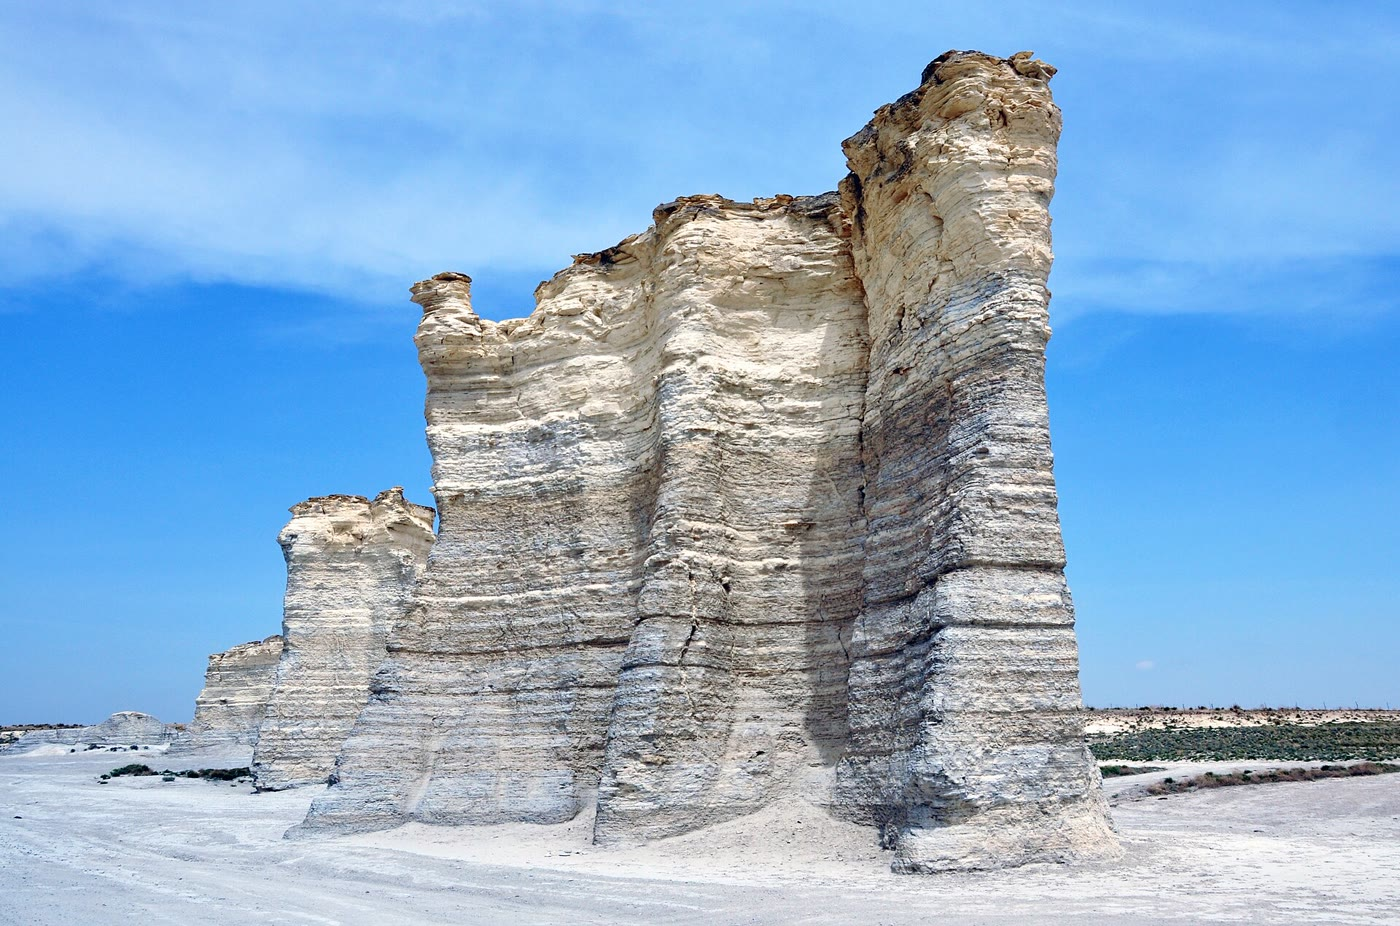
\includegraphics[width=0.66\linewidth]{images/book4/b2-19-monument-rocks.jpg}
\par\smallskip{\small Monument Rocks, oeste de Kansas: pilares de creta, el fango de un mar interior
cretácico de unos 80 millones de años, depositado a unos \qty{0.036}{mm} al año. (James
St.~John, CC~BY~2.0, a través de Wikimedia Commons.)}
\end{omfigure}
% ledger: kgs:monument-rocks, kgs:chalk

\begin{definition}[Mar epicontinental]\label{def:b2:phanerozoic-earth:epeiric}
Un \emph{mar epicontinental}\index{mar epicontinental} es un mar somero extendido sobre el interior de un
continente, sobre corteza continental, lejos del margen continental.
\end{definition}

El mar llega a esos interiores desplazando su costa, y las rocas registran ese desplazamiento.

\begin{definition}[Transgresión marina; regresión marina]\label{def:b2:phanerozoic-earth:transgression}
Una \emph{transgresión marina}\index{transgresion marina@transgresión marina} es un desplazamiento de la línea de costa hacia tierra,
por el que el mar se extiende sobre el continente; una \emph{regresión marina}\index{regresion marina@regresión marina} es
un desplazamiento hacia el mar, por el que emerge la tierra.
\end{definition}

En un corte vertical, una transgresión apila depósitos de aguas más profundas sobre otros más someros
---fango de plataforma sobre arena de playa---, y una regresión, lo contrario. Ambas siguen el nivel relativo
del mar, que mezcla el nivel del mar global con la subsidencia o el levantamiento del lugar y con el
aporte de sedimento: un delta puede empujar su costa hacia el mar mientras el mar sube, si se alimenta con suficiente
rapidez. Para leer el nivel del mar global en las transgresiones, un geólogo debe encontrar la misma señal
en varios continentes, o eliminar la subsidencia por \omterm{def:b2:basins-compared:backstripping}{backstripping}, como en el
\cref{ch:b2:basins-compared}.
% ledger: miller20:rsl

\subsection*{La curva a largo plazo}

\begin{definition}[Ciclo del nivel del mar de primer orden]\label{def:b2:phanerozoic-earth:first-order}
El \emph{ciclo del nivel del mar de primer orden}\index{ciclo del nivel del mar de primer orden} es la parte más lenta
del cambio del nivel del mar global, en escalas de tiempo de decenas a centenares de millones de años, fijada por
la tectónica de la Tierra sólida y no por el hielo.
\end{definition}

A lo largo del Fanerozoico la curva de primer orden tiene forma de M: alta a comienzos del Paleozoico,
baja mientras Pangea se ensamblaba y permanecía unida, del Carbonífero al final del Triásico, alta
de nuevo en el Cretácico, y en descenso desde entonces. Extrapolada a partir de Norteamérica, la inundación del Ordovícico
Superior sugiere por sí sola una subida adicional de 100 a \qty{200}{m}.
Sobre esta curva se superponen cambios más rápidos: los debidos al hielo quedan registrados en escalas de tiempo de $10^4$ a
$10^6$ años, y el casquete antártico, desde unos \qty{33.5}{Ma}, desplazó el mar de 50 a
\qty{60}{m}.
% ledger: th23:flooding, miller11:greenhouse, miller05:abstract

\begin{omfigure}
\centering
% figdata/bachelor-2/phanerozoic.py parts sealevel-haq, sealevel-haqlt, sealevel-kominz, sealevel-kominzlt
\begin{tikzpicture}
\begin{axis}[width=0.92\linewidth, height=6.2cm, x dir=reverse, xmin=0, xmax=252,
  ymin=-130, ymax=280, xlabel={edad (\unit{Ma})}, ylabel={nivel del mar sobre el actual (\unit{m})},
  xtick={0,50,...,250}, ytick={-100,-50,...,250}, xtick pos=bottom, ytick pos=left,
  tick label style={font=\scriptsize}, label style={font=\small},
  legend style={at={(0.5,1.04)}, anchor=south, draw=none, font=\scriptsize, legend columns=2,
  /tikz/every even column/.append style={column sep=8pt}}]
\addplot[black!30, line width=0.3pt] table[x=age_ma, y=sl_m]
  {figdata/out/bachelor-2-phanerozoic-sealevel-haq.dat};
\addlegendentry{Haq y otros (1987)}
\addplot[omThm, line width=0.3pt] table[x=age_ma, y=sl_m]
  {figdata/out/bachelor-2-phanerozoic-sealevel-kominz.dat};
\addlegendentry{Nueva Jersey, backstripping}
\addplot[black, line width=1.2pt] table[x=age_ma, y=sl_m]
  {figdata/out/bachelor-2-phanerozoic-sealevel-haqlt.dat};
\addlegendentry{Haq, media de 10 Myr}
\addplot[omThm!70!black, line width=1.2pt] table[x=age_ma, y=sl_m]
  {figdata/out/bachelor-2-phanerozoic-sealevel-kominzlt.dat};
\addlegendentry{Nueva Jersey, media de 10 Myr}
\addplot[black!50, line width=0.3pt, forget plot] coordinates {(0,0) (252,0)};
\foreach \a/\b/\c in {251.902/201.4/icsTriassic, 201.4/143.1/icsJurassic,
  143.1/66/icsCretaceous, 66/23.04/icsPaleogene, 23.04/2.58/icsNeogene, 2.58/0/icsQuaternary} {
  \edef\tmp{\noexpand\fill[\c] (axis cs:\a,-130) rectangle (axis cs:\b,-112);}\tmp}
\node[font=\tiny, text=white] at (axis cs:226.7,-121) {Triásico};
\node[font=\tiny, text=white] at (axis cs:172.3,-121) {Jurásico};
\node[font=\tiny] at (axis cs:104.6,-121) {Cretácico};
\node[font=\tiny] at (axis cs:44.5,-121) {Paleógeno};
\node[font=\tiny] at (axis cs:12.8,-121) {Neóg.};
\end{axis}
\end{tikzpicture}
\par\smallskip{\small Nivel del mar global desde \qty{250}{Ma}, según la tabulación de Miller y otros
(2005): la carta de ciclos de Haq y otros (1987), a partir de la estratigrafía de numerosas cuencas, y el
nivel del mar obtenido por \omterm{def:b2:basins-compared:backstripping}{backstripping} de sondeos de Nueva Jersey, con niveles bajos estimados (Kominz y
otros 2008). Líneas gruesas: medias móviles de 10 Myr, la tendencia de primer orden. Edades en la escala
de tiempo de 2012; la barra inferior muestra los periodos.}
\end{omfigure}
% ledger: data:b4-sealevel, haq87:charts, kominz08:long-term, ics:base.Triassic, ics:base.Jurassic, ics:base.Cretaceous, ics:base.Paleogene, ics:base.Neogene, ics:base.Quaternary, ics:colour.Triassic, ics:colour.Jurassic, ics:colour.Cretaceous, ics:colour.Paleogene, ics:colour.Neogene, ics:colour.Quaternary

Las dos curvas anteriores coinciden en la forma y discrepan en el tamaño. La carta de ciclos, construida a partir del
apilamiento de sedimentos en numerosas cuencas, sitúa el nivel del mar a largo plazo del Cretácico medio
unos \qty{233}{m} por encima del actual; los sondeos de Nueva Jersey, sometidos uno a uno a \omterm{def:b2:basins-compared:backstripping}{backstripping}, dan unos
\qty{70}{m} en el Cretácico Superior y un máximo cercano a \qty{110}{m} en el Eoceno. Miller y sus
colegas concluyen que el máximo cretácico a largo plazo fue de $100 \pm \qty{50}{m}$, y que las
cartas de ciclos, acertadas en la cronología de los descensos, exageran sus amplitudes. Ni siquiera Nueva Jersey
es un indicador perfecto: su mar del Cretácico Superior está de 100 a \qty{150}{m} por debajo de lo que predice el volumen de
las cuencas oceánicas, una diferencia que podría explicarse por el hundimiento de la región sobre la placa subducida de
Farallón ---la topografía dinámica---.
% ledger: data:b4-sealevel, miller05:abstract, kominz08:long-term, miller20:epr

\subsection*{Por qué se mueve el mar: las dorsales}

¿Qué hace subir el mar un centenar de metros durante decenas de millones de años? No el hielo: el Cretácico
fue un mundo cálido con, como mucho, casquetes de hielo pequeños y efímeros. La respuesta principal es el volumen de
las dorsales oceánicas. El fondo oceánico joven es caliente y está elevado; cuanto más deprisa se separan las placas, más
joven es en promedio el fondo, menos profundas son las cuencas oceánicas y más agua se desborda sobre
los continentes.
% ledger: miller11:greenhouse, th23:pitman

\begin{proposition}[Nivel del mar y velocidad de expansión]\label{prop:b2:phanerozoic-earth:ridge}
Fórmese fondo oceánico de área $A_{\text{f}}$ en dorsales de longitud total $L$ a la velocidad de expansión
total $u$, y destrúyase a la edad $\tau = A_{\text{f}}/(Lu)$, de modo que cada edad entre 0
y $\tau$ cubra la misma área. Siga su profundidad la ley $d(t) = d_{\text{r}} + c\sqrt t$.
\begin{enumerate}
  \item La profundidad media del fondo es $\bar d = d_{\text{r}} + \tfrac23 c\sqrt\tau$.
  \item Si la velocidad de expansión pasa a ser $fu$, con $A_{\text{f}}$ y $L$ sin cambios, la profundidad
        media disminuye en $\Delta\bar d = \tfrac23 c\sqrt\tau\,\bigl(1 - f^{-1/2}\bigr)$.
  \item Si el fondo se hunde isostáticamente bajo el agua añadida, y el mar no se extiende
        sobre la tierra, el nivel del mar sobre un océano de área $A_{\text{o}}$ sube
        \[
        \Delta s = \frac{\rho_{\text{m}} - \rho_{\text{w}}}{\rho_{\text{m}}}\,
        \frac{A_{\text{f}}}{A_{\text{o}}}\,\Delta\bar d ,
        \]
        con $\rho_{\text{m}}$ la densidad del manto y $\rho_{\text{w}}$ la del agua de mar.
\end{enumerate}
\end{proposition}

\begin{proof}
(1) Las dorsales crean fondo nuevo al ritmo $Lu$ (área por unidad de tiempo), y cada franja de fondo vive
durante el tiempo $\tau$; en régimen estacionario, el área de fondo con edad entre $t$ y $t + \mathrm{d}t$
es $Lu\,\mathrm{d}t$ para todo $t < \tau$, así que el área total es $Lu\tau = A_{\text{f}}$ y las
edades están repartidas uniformemente. La profundidad media es
$\frac1\tau\int_0^\tau (d_{\text{r}} + c\sqrt t)\,\mathrm{d}t = d_{\text{r}} + \frac{c}{\tau}
\cdot\frac23\tau^{3/2}$. (2) Con la velocidad $fu$, $\tau$ pasa a ser $\tau/f$, y
$\sqrt{\tau/f} = f^{-1/2}\sqrt\tau$. (3) Las cuencas pierden el volumen $\Delta V = A_{\text{f}}
\Delta\bar d$. Suba la superficie del mar $\Delta s$ respecto de los continentes, y húndase el fondo
$y$ bajo el agua adicional. La columna de agua adicional, de espesor $\Delta s + y$, sustituye a un
espesor $y$ de manto en el equilibrio isostático: $\rho_{\text{w}}(\Delta s + y) =
\rho_{\text{m}} y$, así que $y = \rho_{\text{w}}\Delta s/(\rho_{\text{m}} - \rho_{\text{w}})$ y
$\Delta s + y = \Delta s\,\rho_{\text{m}}/(\rho_{\text{m}} - \rho_{\text{w}})$. El volumen se
conserva: $A_{\text{o}}(\Delta s + y) = \Delta V$, lo que da el resultado.
\end{proof}

El fondo real no es tan ordenado. Sus edades no están repartidas uniformemente: el fondo joven es el más abundante,
y el área disminuye con la edad, como muestra el panel izquierdo siguiente. Tampoco se cumple la ley de la raíz cuadrada en el
fondo antiguo, que se aplana cerca de \qty{6.4}{km}; la ley exponencial que Parsons y Sclater
ajustaron al fondo antiguo, la ley de la placa, toma el relevo más allá de unos \qty{26}{Myr}, donde las dos leyes
se encuentran. La proposición es una primera estimación, y la figura
muestra cuánto la cambia la segunda ley.
% ledger: ps77:depth-age, data:b4-ridge

\begin{omfigure}
\centering
% figdata/bachelor-2/phanerozoic.py parts agehist and ridge
\begin{tikzpicture}
\begin{groupplot}[group style={group size=2 by 1, horizontal sep=1.6cm},
  width=0.5\linewidth, height=5.6cm, tick label style={font=\scriptsize},
  label style={font=\small}, xtick pos=bottom, ytick pos=left]
\nextgroupplot[xmin=0, xmax=200, ymin=0, ymax=34, xlabel={edad del fondo (\unit{Myr})},
  ylabel={área por cada \qty{10}{Myr} (\unit{\mega km^2})},
  legend style={at={(0.5,1.04)}, anchor=south, draw=none, font=\scriptsize}]
\addplot[ybar interval, area legend, fill=omSea!80!black, draw=black!50, line width=0.2pt]
  table[x expr=\thisrow{age}-5, y=area_Mkm2] {figdata/out/bachelor-2-phanerozoic-agehist.dat};
\addlegendentry{malla de edades}
\addplot[const plot mark mid, black, dashed, line width=0.9pt]
  table[x=age, y=uniform_Mkm2] {figdata/out/bachelor-2-phanerozoic-agehist.dat};
\addlegendentry{edades uniformes hasta \qty{128.4}{Myr}}
\nextgroupplot[xmin=1, xmax=3, ymin=0, ymax=650, xlabel={velocidad de expansión / actual, $f$},
  ylabel={subida del nivel del mar $\Delta s$ (\unit{m})},
  legend style={at={(0.5,1.04)}, anchor=south, draw=none, font=\scriptsize, legend columns=2}]
\fill[omThm!15] (axis cs:1,50) rectangle (axis cs:3,150);
\addplot[black, line width=1pt] table[x=f, y=ds_hs] {figdata/out/bachelor-2-phanerozoic-ridge.dat};
\addlegendentry{ley $\sqrt t$}
\addplot[blue!70!black, dashed, line width=1pt] table[x=f, y=ds_plate]
  {figdata/out/bachelor-2-phanerozoic-ridge.dat};
\addlegendentry{ley de la placa}
\node[font=\scriptsize, anchor=west] at (axis cs:1.6,100) {$100 \pm \qty{50}{m}$};
\end{groupplot}
\end{tikzpicture}
\par\smallskip{\small Izquierda: área del fondo oceánico actual en intervalos de edad de 10 Myr, a partir de la malla de edades
de Seton y otros (2020) con una resolución de un grado (\qty{293}{\mega km^2} en total), frente al
reparto uniforme de la \cref{prop:b2:phanerozoic-earth:ridge} con la misma área y la misma edad media. Derecha:
subida del nivel del mar cuando la velocidad de expansión se multiplica por $f$, según la proposición con la
ley de la raíz cuadrada y con la ley de la placa, partiendo del reparto uniforme hasta \qty{128.4}{Myr}; la
banda es el máximo cretácico a largo plazo estimado por Miller y otros (2005).}
\end{omfigure}
% ledger: data:b4-ridge, data:b2-seafloor-age, seton:mean-age, ps77:depth-age, miller05:abstract, charette:ocean-volume, katz03:thermo, noaa:seawater-1025

\begin{example}[El doble de rápido]\label{ex:b2:phanerozoic-earth:doubling}
Tómese el fondo actual: edad media \qty{64.2}{Myr}, así que $\tau = \qty{128.4}{Myr}$ en el modelo uniforme;
$d_{\text{r}} = \qty{2500}{m}$, $c = \qty{350}{m.Myr^{-1/2}}$. La profundidad media es $2500 + \tfrac23
\times 350 \times \sqrt{128.4} = \qty{5144}{m}$. Duplicar la velocidad reduce $\tau$ a la mitad, y la profundidad
media pasa a ser $2500 + \tfrac23 \times 350 \times \sqrt{64.2} = \qty{4370}{m}$: el fondo sube en promedio
\qty{774}{m}. Con $A_{\text{f}}/A_{\text{o}} = 293/362 = 0.8094$ y
$(\rho_{\text{m}} - \rho_{\text{w}})/\rho_{\text{m}} = (3300 - 1025)/3300 = 0.689$, el mar sube
$0.689 \times 0.8094 \times 774 = \qty{432}{m}$; con la ley de la placa, \qty{368}{m}. Ambos valores son
unas cuatro veces el máximo cretácico a largo plazo. Leído al revés, el panel derecho dice que una
velocidad de expansión solo de un 15 a un \qty{20}{\percent} superior a la actual basta para \qty{100}{m} ---por
eso Miller y sus colegas concluyen que la corteza oceánica se formó mucho más despacio en el
Cretácico de lo que se había deducido---.
\end{example}
% ledger: seton:mean-age, ps77:depth-age, data:b4-ridge, charette:ocean-volume, katz03:thermo, noaa:seawater-1025, miller05:abstract
% values (phanerozoic.py numbers): dbar_hs 5144, dbar_hs_half 4369.6, rise2_hs 432.5, rise2_pl 368.4, f_for_100_hs 1.151

El modelo es además demasiado profundo: su profundidad media, \qty{5144}{m}, supera la profundidad media medida del
fondo datado, \qty{4265}{m}, en parte porque la ley de la raíz cuadrada se excede en el fondo antiguo, y
en parte porque el fondo real lleva sedimento, \omterm{def:b2:oceanic-islands:seamount}{montes submarinos} y mesetas que la ley deja fuera. Y la expansión no es la
única palanca. Las dorsales están compensadas por las fosas: si el fondo oceánico sube en un lugar, la masa tiene que
ir a alguna parte, y un continente que se hunde sobre una placa subducida ---la topografía dinámica--- deja entrar el mar
localmente. Tasistro-Hart y Macdonald sostienen que las inundaciones de Norteamérica siguen a las placas subducidas
bajo el continente, y que el nivel del mar global depende de cuánta subducción se produce bajo los
continentes y no bajo los océanos.
% ledger: data:b4-floor-depth, th23:pitman, th23:flooding, kominz08:long-term

\section{La inundación de los continentes}\label{sec:b2:phanerozoic-earth:flooding}

Cuánta tierra ahoga una subida del mar depende de la forma de la superficie terrestre, que resume la
curva hipsométrica del volumen de primer año: la fracción de la superficie que está por encima de
cada altitud (figura siguiente, a la izquierda). Los continentes tienen la cima plana. En la malla de un grado de
ETOPO1, el \qty{29.0}{\percent} de la superficie es tierra emergida y el \qty{34.3}{\percent} está por encima de
\qty{-200}{m}: las plataformas, ya bajo el agua, marcan la diferencia. La mayor parte de la tierra es baja, de modo que una
subida modesta inunda una gran parte de ella.
% ledger: data:b4-hyps, data:etopo1

\begin{proposition}[La inundación de la tierra]\label{prop:b2:phanerozoic-earth:flooding}
Sean $A_{\text{o}}$ el área actual del mar y $a(z)$ el área de tierra situada a menos de $z$ sobre el
nivel del mar actual. Un volumen $V$ de agua añadido al mar eleva su nivel hasta la altura $s$
que cumple
\[
V = \int_0^s \bigl(A_{\text{o}} + a(z)\bigr)\,\mathrm{d}z ,
\]
e inunda el área de tierra $a(s)$. Como $a \ge 0$, la subida es como mucho $V/A_{\text{o}}$.
\end{proposition}

\begin{proof}
Cuando el mar está a $z$, cubre $A_{\text{o}} + a(z)$; elevarlo $\mathrm{d}z$ requiere
el volumen $\bigl(A_{\text{o}} + a(z)\bigr)\mathrm{d}z$. Sumando de 0 a $s$ se obtiene $V$. El
integrando es al menos $A_{\text{o}}$, así que $V \ge A_{\text{o}}s$.
\end{proof}

\begin{omfigure}
\centering
% figdata/bachelor-2/phanerozoic.py parts hyps and flood
\begin{tikzpicture}
\begin{groupplot}[group style={group size=2 by 1, horizontal sep=1.6cm},
  width=0.46\linewidth, height=5.6cm, tick label style={font=\scriptsize},
  label style={font=\small}, xtick pos=bottom, ytick pos=left]
\nextgroupplot[xmin=0, xmax=100, ymin=-9500, ymax=6500,
  xlabel={porcentaje de la superficie por encima de $z$}, ylabel={altitud $z$ (\unit{m})},
  scaled y ticks=false, yticklabel style={/pgf/number format/1000 sep={\,}}]
\addplot[omThm, line width=1pt] table[x=pct, y=z] {figdata/out/bachelor-2-phanerozoic-hyps.dat};
\addplot[black!50, line width=0.3pt] coordinates {(0,0) (100,0)};
\node[font=\scriptsize, anchor=south west] at (axis cs:30,100) {tierra \qty{29.0}{\percent}};
\node[font=\scriptsize] at (axis cs:45,-7000) {fondo oceánico};
\nextgroupplot[xmin=0, xmax=1000, ymin=0, ymax=80, xlabel={subida del nivel del mar $h$ (\unit{m})},
  ylabel={tierra inundada (\unit{\percent})}]
\addplot[omThm, line width=1pt] table[x=h, y=flooded_pct]
  {figdata/out/bachelor-2-phanerozoic-flood.dat};
\addplot[black, dashed, line width=0.5pt] coordinates {(100,0) (100,14.9) (0,14.9)};
\addplot[black, dashed, line width=0.5pt] coordinates {(432,0) (432,50.6) (0,50.6)};
\end{groupplot}
\end{tikzpicture}
\par\smallskip{\small Izquierda: curva hipsométrica de la Tierra a partir de la malla ETOPO1 de un grado.
Derecha: porcentaje de la tierra actual situada por debajo de cada altura sobre el nivel del mar, la tierra que inundaría una subida $h$
si nada más se moviera; las líneas discontinuas marcan \qty{100}{m} y \qty{432}{m}. Promediar sobre
celdas de un grado suaviza el relieve, así que son primeras estimaciones.}
\end{omfigure}
% ledger: data:b4-hyps, data:etopo1

El panel derecho da la respuesta de inmediato. Una subida de \qty{100}{m} ahoga alrededor del
\qty{15}{\percent} de la tierra actual; los \qty{432}{m} de una velocidad de expansión duplicada ahogarían la
mitad. Un mar así se extiende sobre la tierra que inunda, de modo que la subida misma es menor que la
cota $V/A_{\text{o}}$ de la proposición, en alrededor de una décima para una subida de unos cientos de metros (problema
de fin de semana). Los mares cretácicos de Kansas necesitaron mucho menos: el interior de un continente suele ser
bajo, y además puede hundirse sobre una placa subducida.
% ledger: data:b4-hyps
% values (phanerozoic.py numbers): flood_100 14.9, flood_rise2 50.8, level_rise2_spread 390.7

\section{Las cordilleras del Fanerozoico}\label{sec:b2:phanerozoic-earth:orogens}

Cada \omterm{def:b2:wilson-cycle:wilson}{ciclo de Wilson} del \cref{ch:b2:wilson-cycle} termina en una cordillera, y las cordilleras
fanerozoicas marcan la formación y la fragmentación de Pangea. La tabla reúne las que han aparecido en este volumen.

\begin{center}
\small
\begin{tabular}{>{\raggedright\arraybackslash}p{0.15\linewidth}>{\raggedright\arraybackslash}p{0.22\linewidth}>{\raggedright\arraybackslash}p{0.22\linewidth}>{\raggedright\arraybackslash}p{0.29\linewidth}}
\hline
orogenia & época & océano cerrado & qué colisionó \\
\hline
caledoniana & c.~540--400 Ma; colisión principal 425--400 Ma & Iapetus & Laurentia, Báltica y
Avalonia, que forman Laurusia \\
varisca--apalachiana & desde c.~550 Ma; colisión final Carbonífero Superior--Pérmico & Rheico &
Gondwana y sus \omterm{def:b2:wilson-cycle:terrane}{terranes} desprendidos con Laurusia, que forman Pangea \\
alpina & Cretácico (máximo hacia 100 Ma) y Cenozoico & Tetis alpino & Apulia y Europa \\
himalaya & desde c.~60 a 54 Ma (discutido) hasta hoy & océano al norte de la India & India y Asia \\
andina & todavía activa; acortamiento desde el Oligoceno & ninguno: subduce una placa oceánica & la
placa de Nazca bajo Sudamérica \\
\hline
\end{tabular}
\end{center}
% ledger: mckerrow00:caledonian, schiffer20:caledonides, schiffer20:variscan, faure24:variscan, usgs:alleghanian-age, schmid04:two-orogenies, najman21:collision-age, gerbault05:andes, nance22:supercontinents

Las dos primeras cordilleras cosieron Pangea, al cerrar la varisca el último océano entre Gondwana
y Laurusia; las tres últimas crecieron a medida que los fragmentos de Pangea se separaban y los océanos entre
ellos se consumían. El nivel del mar bajo del Paleozoico superior y del Triásico corresponde a este
\omterm{def:b2:wilson-cycle:supercontinent}{supercontinente}, y el mar alto del Cretácico a su fragmentación, con dorsales nuevas y fondo
joven.
% ledger: schiffer20:variscan, th23:flooding, nance22:supercontinents

\section{Crisis de la vida}\label{sec:b2:phanerozoic-earth:extinctions}

\subsection*{Las cinco grandes}

Los volúmenes de biología describen las extinciones masivas; los geólogos las miden en las rocas y buscan
sus causas. Cinco destacan en el registro de los animales marinos, las «cinco grandes»: al final del
Ordovícico, hace unos \qty{444}{Ma}; en el Devónico Superior, \qty{372}{Ma}; al final del Pérmico,
\qty{251.9}{Ma}; al final del Triásico, \qty{201.4}{Ma}; y al final del Cretácico,
\qty{66}{Ma}. Cada una eliminó entre unas dos quintas partes y dos tercios de los géneros de animales
marinos de la compilación de Sepkoski. La crisis del final del Pérmico fue la mayor: el \qty{56}{\percent} de los
géneros con la resolución más fina, y alrededor del \qty{81}{\percent} de las especies marinas ---no el
\qty{96}{\percent} que se cita a menudo, que mezclaba dos crisis distintas---.
% ledger: kaiho22:table, marshall23:big-five, stanley16:permian

\begin{history}[Las cinco grandes, cuarenta años después]
En 1982, D.~M.~Raup y J.~J.~Sepkoski contaron las familias de animales marinos que desaparecieron
en cada uno de 76 pisos del Fanerozoico. Cuatro puntos quedaban por encima del límite de confianza del 99~por ciento
de su tendencia ---el último piso del Ordovícico, los dos últimos del Pérmico y el último del
Cretácico--- y el final del Triásico y el final del Devónico, por encima del límite del 95~por
ciento: las cinco grandes. Cuarenta años después, las cinco siguen siendo las mayores crisis desde el Ordovícico
inferior, pero con mejores datos ya no se separan de un continuo de tasas de
extinción, y algunos intervalos del Cámbrico tuvieron tasas incluso más altas. La resolución temporal de Raup y Sepkoski
era de \qty{7.4}{Myr}, la duración media de un piso entonces; algunas crisis fueron repentinas, otras
duraron cientos de miles de años o más.
\end{history}
% ledger: marshall23:big-five, marshall23:resolution

\begin{omfigure}
\centering
% figdata/bachelor-2/phanerozoic.py parts ext, lip, oae
\begin{tikzpicture}
\begin{axis}[width=0.95\linewidth, height=6.4cm, x dir=reverse, xmin=0, xmax=541,
  ymin=-34, ymax=80, xlabel={edad (\unit{Ma})}, ylabel={géneros marinos perdidos (\unit{\percent})},
  xtick={0,100,...,500}, ytick={0,20,...,80}, xtick pos=bottom, ytick pos=left,
  tick label style={font=\scriptsize}, label style={font=\small}, clip=false]
\addplot[ybar, bar width=5pt, fill=omThm!70, draw=black!60]
  % etiquetas: nodos explícitos (la tabla figdata lleva los nombres en inglés)
  table[x=age, y=value] {figdata/out/bachelor-2-phanerozoic-ext.dat}; \foreach \a/\v/\t in {444/52/fin del Ordovícico, 372/41/Devónico Superior, 251.9/66/fin del Pérmico, 201.4/46/fin del Triásico, 66/45/fin del Cretácico} {\edef\temp{\noexpand\node[font=\noexpand\tiny, anchor=south] at (axis cs:\a,\v) {\t};}\temp}
\addplot[only marks, mark=triangle*, mark size=2.6pt, red!70!black]
  table[x=age, y expr=-6] {figdata/out/bachelor-2-phanerozoic-lip.dat};
\addplot[only marks, mark=diamond*, mark size=2.6pt, blue!70!black]
  table[x=age, y expr=-13] {figdata/out/bachelor-2-phanerozoic-oae.dat};
\addplot[only marks, mark=star, mark size=4pt, line width=1pt, black] coordinates {(66,-20)};
\node[font=\tiny, anchor=west, red!70!black] at (axis cs:541,-6) {GPI};
\node[font=\tiny, anchor=west, blue!70!black] at (axis cs:541,-13) {OAE};
\node[font=\tiny, anchor=west] at (axis cs:541,-20) {impacto};
\node[font=\tiny, anchor=west] at (axis cs:57,-20) {Chicxulub};
\foreach \a/\b/\c in {538.8/486.85/icsCambrian, 486.85/443.1/icsOrdovician,
  443.1/419.62/icsSilurian, 419.62/358.86/icsDevonian, 358.86/298.9/icsCarboniferous,
  298.9/251.902/icsPermian, 251.902/201.4/icsTriassic, 201.4/143.1/icsJurassic,
  143.1/66/icsCretaceous, 66/23.04/icsPaleogene, 23.04/2.58/icsNeogene, 2.58/0/icsQuaternary} {
  \edef\tmp{\noexpand\fill[\c] (axis cs:\a,-34) rectangle (axis cs:\b,-27);}\tmp}
\foreach \x/\t in {512.8/Cm, 465/O, 431.4/S, 389.2/D, 328.9/C, 275.4/P, 226.7/Tr, 172.3/J,
  104.6/K, 44.5/Pg, 12.8/N} {
  \edef\tmp{\noexpand\node[font=\noexpand\tiny] at (axis cs:\x,-30.5) {\t};}\tmp}
\end{axis}
\end{tikzpicture}
\par\smallskip{\small Las cinco grandes extinciones masivas, con la proporción de géneros marinos perdidos en
la compilación de Sepkoski (Kaiho 2022, tabla~1), las grandes provincias ígneas (GPI; triángulos, edades medias de
Courtillot y Renne 2003, desde \qty{259}{Ma}), los \omterm{def:b2:phanerozoic-earth:oae}{eventos anóxicos oceánicos} mejor estudiados
(OAE; rombos) y el impacto de Chicxulub. La barra inferior muestra los periodos.}
\end{omfigure}
% ledger: kaiho22:table, cr03:table, rigo24:oaes, pickersgill26:chicxulub, ics:base.Cambrian, ics:base.Ordovician, ics:base.Silurian, ics:base.Devonian, ics:base.Carboniferous, ics:base.Permian, ics:base.Triassic, ics:base.Jurassic, ics:base.Cretaceous, ics:base.Paleogene, ics:base.Neogene, ics:base.Quaternary, ics:colour.Cambrian, ics:colour.Ordovician, ics:colour.Silurian, ics:colour.Devonian, ics:colour.Carboniferous, ics:colour.Permian

\subsection*{Grandes provincias ígneas}

La figura anterior muestra la pauta que señalaba el volumen de primer año: las tres más recientes de
las cinco grandes coinciden cada una con una gran provincia ígnea, los traps de Siberia al final del Pérmico,
la Provincia Magmática del Atlántico Central (CAMP) al final del Triásico, los traps del Decán al
final del Cretácico. El vínculo propuesto es el gas. Un basalto de inundación entra en erupción en pulsos de unos pocos
siglos a unos pocos milenios, cada uno de los cuales libera dióxido de carbono más deprisa de lo que la meteorización puede
retirarlo; el azufre de las mismas erupciones enfría brevemente el clima, el carbono lo calienta durante mucho
más tiempo y acidifica el océano.
% ledger: cr03:table, cr03:summary, capriolo20:camp-co2

\begin{example}[El carbono de la provincia del Atlántico Central]\label{ex:b2:phanerozoic-earth:camp}
Las burbujas de gas de las inclusiones fundidas de los basaltos de la CAMP muestran que el \omterm{def:b2:magma-emplacement:magma}{magma} contenía al menos del 0.5 al
\qty{0.6}{\percent} de dióxido de carbono en masa. Tómense un \qty{0.55}{\percent}, una densidad de
\qty{2900}{kg.m^{-3}} y un volumen de \qty{5.5e6}{km^3}, las lavas emitidas con los \omterm{def:b2:magma-emplacement:bodies}{diques}, sills
y cámaras que las alimentaron. La masa de \omterm{def:b2:magma-emplacement:magma}{magma} es $\num{5.5e6} \times \num{e9} \times 2900 =
\qty{1.6e19}{kg}$, y su dióxido de carbono, $\num{1.6e19} \times 0.0055 = \qty{8.8e16}{kg}$, unas
\qty{9e4}{Gt} ---el «hasta \qty{e5}{Gt}» de los autores---. Liberado a lo largo de la vida de la provincia, no
estuvo todo en el aire a la vez; pero cada pulso, del orden de \qty{e5}{km^3} en unos pocos
siglos, liberó tanto como las emisiones proyectadas para el siglo XXI.
\end{example}
% ledger: capriolo20:camp-co2
% values: 5.5e6 km3 x 2900 kg/m3 = 1.595e19 kg; x 0.0055 = 8.77e16 kg

\subsection*{Eventos anóxicos oceánicos}

No toda crisis es una de las cinco grandes. Varias veces en el Mesozoico, el oxígeno desapareció de
grandes partes del océano.

\begin{definition}[Evento anóxico oceánico]\label{def:b2:phanerozoic-earth:oae}
Un \emph{evento anóxico oceánico}\index{evento anoxico oceanico@evento anóxico oceánico} (OAE, por sus siglas en inglés) es un intervalo de agotamiento generalizado
del oxígeno en el océano, reconocido en el registro sedimentario y geoquímico.
\end{definition}

Su marca habitual es una lutita negra: oscura, finamente laminada, sin bioturbación, rica en materia orgánica
y en pirita, a menudo con un desplazamiento de los isótopos del carbono y señales de calentamiento. Los mejor estudiados
son el evento del Toarciense inferior, hacia \qty{183}{Ma}, el OAE~1a del Aptiense inferior, hacia \qty{120}{Ma},
el OAE~1b del Albiense inferior, hacia \qty{111}{Ma}, y el OAE~2 en el límite entre el Cenomaniense
y el Turoniense, hacia \qty{94}{Ma}, en la parte más cálida del Cretácico, cuando el mar estaba
excepcionalmente alto. Varios coinciden con una provincia: el evento toarciense con los basaltos de Karoo--Ferrar,
el OAE~1a con la meseta de Ontong Java. El OAE~2 suele relacionarse con la meseta del Caribe, pero
los picos de mercurio en sedimentos del hemisferio sur apuntan en cambio a la provincia de Kerguelen.
% ledger: rigo24:oaes, wt24:oae2, cr03:table

\begin{omfigure}
\centering
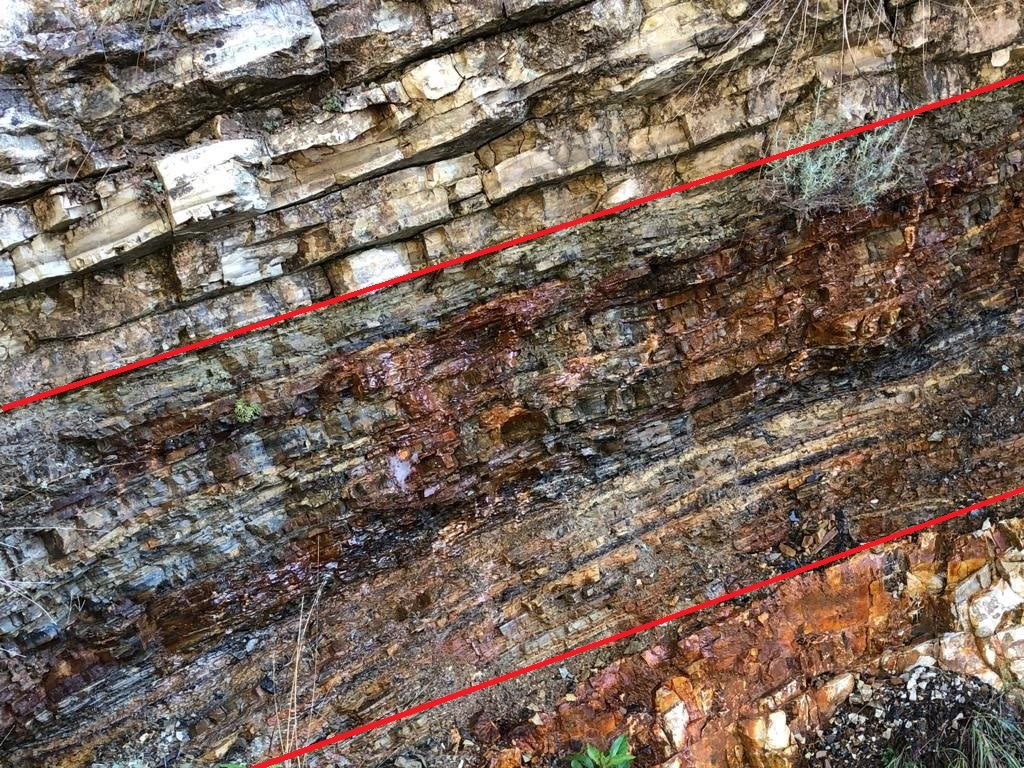
\includegraphics[width=0.66\linewidth]{images/book4/b2-19-bonarelli-level.jpg}
\par\smallskip{\small El nivel Bonarelli, la lutita oscura del OAE~2, entre calizas claras; las
líneas rojas, trazadas por el fotógrafo, marcan su base y su techo. (Picenus, CC~BY-SA~4.0, a través de
Wikimedia Commons.)}
\end{omfigure}
% ledger: rigo24:oaes

\begin{inthefield}[Levantar la columna de un evento anóxico]
Una geóloga que estudia un OAE en una sección de calizas pelágicas la levanta capa a capa: espesor,
color, laminación, bioturbación o su ausencia, nódulos de pirita. Muestrea a intervalos cortos y regulares
a través del intervalo oscuro y bastante más allá, para el contenido en carbono orgánico y para los
isótopos del carbono de la materia orgánica y del carbonato; el desplazamiento de los isótopos, más que
el color de la roca, correlaciona el evento de una cuenca a otra. Como la lutita más oscura
puede aparecer a niveles distintos en cuencas distintas, se toma como línea de tiempo la curva isotópica, no la lutita
negra.
\end{inthefield}
% ledger: rigo24:oaes, wt24:oae2

\subsection*{Chicxulub}

El final del Cretácico tuvo una causa exterior. El volumen de primer año contó cómo el iridio de la
arcilla del límite llevó a un impacto, y cómo la datación por argón vinculó el límite al cráter de Chicxulub.
La estructura tiene unos \qty{200}{km} de diámetro y \qty{66}{Ma} de antigüedad; sus
rocas calientes alimentaron la circulación de agua durante al menos ocho millones de años después. Los modelos de su asimetría
en el subsuelo apuntan a un impactor que llegó del nordeste con una inclinación de 45 a \ang{60} sobre la horizontal,
a no menos de la velocidad de escape de la Tierra, \qty{11.2}{km.s^{-1}}, y más probablemente a unos
\qty{20}{km.s^{-1}}. Los traps del Decán estaban en erupción al mismo tiempo, antes y después del
impacto; una revisión de las pruebas publicada en 2010 concluyó que el impacto desencadenó la extinción.
% ledger: pickersgill26:chicxulub, collins20:impact, renne:kpg, alvarez:iridium, schulte:kpg, cr03:deccan

\begin{dated}{2026}
Las edades de este capítulo son las de la Tabla Cronoestratigráfica Internacional en su versión de junio
de 2026, como en toda esta serie; los registros del nivel del mar están en la escala de tiempo de 2012
de sus ficheros, y las edades de las extinciones son las de Kaiho (2022). La tabla se revisa a medida que llegan
nuevas dataciones: compruébese la versión vigente antes de citar la edad de un límite.
\end{dated}
% ledger: ics:base.Phanerozoic, data:b4-sealevel, kaiho22:table

\section*{Ejercicios}\label{sec:b2:phanerozoic-earth:exercises}

Datos para los ejercicios, salvo indicación contraria: \qty{111.2}{km} por grado de latitud; profundidad
del fondo oceánico $d(t) = 2500 + 350\sqrt t$ (\unit{m}, $t$ en \unit{Myr}); área del océano
\qty{362}{\mega km^2}; área del fondo oceánico \qty{293}{\mega km^2}; densidad del manto
\qty{3300}{kg.m^{-3}}; agua de mar \qty{1025}{kg.m^{-3}}; masa de la atmósfera
\qty{5.1e18}{kg}, masas molares del aire y del dióxido de carbono \qty{28.97}{g.mol^{-1}} y
\qty{44.01}{g.mol^{-1}}.
% ledger: earth:Rmean, ps77:depth-age, charette:ocean-volume, data:b4-ridge, katz03:thermo, noaa:seawater-1025, earth:Matm, earth:Mmol, ciaaw:abridged-2024

\begin{exercise}[$\star$]\label{exo:b2:phanerozoic-earth:1}
En el modelo de los mapas, Ciudad del Cabo estaba a \ang{61.9}~S hace \qty{300}{Ma} y Nueva York a
\ang{3.6}~S; hoy están a \ang{33.9}~S y \ang{40.7}~N. (a) ¿Cuáles de las cuatro ciudades estaban
a menos de \ang{30} del ecuador hace \qty{300}{Ma} (París a \ang{5.1}~N, Sídney a
\ang{59.5}~S)? (b) ¿Cuántos kilómetros hacia el norte se han desplazado desde entonces Ciudad del Cabo y Nueva York?
(c) ¿A qué velocidades medias, en centímetros al año?
\end{exercise}
% ledger: data:b4-palaeopos, geonames4:cities

\begin{exercise}[$\star$]\label{exo:b2:phanerozoic-earth:2}
Las cinco grandes ocurrieron hace 444, 372, 251.9, 201.4 y \qty{66}{Ma}. (a) Hállense los intervalos entre
crisis sucesivas y su media. (b) Con las edades medias de las grandes provincias ígneas
---Emeishan 259, Siberia 250, CAMP 201, Karoo--Ferrar 183, Decán \qty{65.5}{Ma}---, ¿cuáles de las
cinco caen a menos de \qty{2}{Myr} de una provincia? (c) ¿Basta un intervalo medio para que las crisis sean periódicas?
\end{exercise}
% ledger: kaiho22:table, cr03:table

\begin{exercise}[$\star$]\label{exo:b2:phanerozoic-earth:3}
La creta de Monument Rocks se depositó a unos \qty{0.036}{mm} al año. (a) ¿Cuánto tardaron en depositarse
\qty{91}{m}? (b) ¿Cuántas veces más deprisa sube hoy el mar, a \qty{3.7}{mm} al
año? (c) ¿Por qué puede un fondo marino recoger una lluvia de sedimento tan lenta sin quedar enterrado por el fango?
\end{exercise}
% ledger: kgs:monument-rocks, ipcc:sea-level-obs

\begin{exercise}[$\star$]\label{exo:b2:phanerozoic-earth:4}
En un acantilado, de abajo arriba: arenisca fluvial con raíces, arena de playa con conchas, fango gris de
plataforma, creta; después, la creta está recubierta de nuevo por arena de playa. (a) ¿Dónde registra la sección una
\omterm{def:b2:phanerozoic-earth:transgression}{transgresión marina}, y dónde una regresión? (b) ¿Demuestra la transgresión que subió el nivel del mar
global? (c) ¿Qué la haría más convincente?
\end{exercise}

\begin{exercise}[$\star\star$]\label{exo:b2:phanerozoic-earth:5}
En la curva a largo plazo de Haq y otros, el nivel del mar estaba \qty{233}{m} por encima del actual hace
\qty{97}{Ma}. (a) ¿Qué velocidad media de descenso desde entonces, en metros por millón de años y en
micrómetros al año? (b) Compárese con la subida actual de \qty{3.7}{mm} al año. (c) La curva de
Nueva Jersey obtenida por \omterm{def:b2:basins-compared:backstripping}{backstripping} da unos \qty{70}{m} en la misma época. ¿De cuál se fiaría usted para la
amplitud, y por qué?
\end{exercise}
% ledger: data:b4-sealevel, ipcc:sea-level-obs, miller05:abstract, miller20:epr

\begin{exercise}[$\star\star$]\label{exo:b2:phanerozoic-earth:6}
Un solo pulso de la CAMP, unos \qty{e5}{km^3} de basalto de densidad \qty{2900}{kg.m^{-3}},
se emitió en unos 500 años. (a) Con un \qty{0.75}{\percent} de dióxido de carbono en masa, ¿cuánto
liberó, en kilogramos y en moles? (b) ¿Qué masa de dióxido de carbono contenía el aire con
las \qty{278}{ppm} de 1750? (c) Compárese. (d) ¿Cuántas atmósferas como esa habría proporcionado toda la provincia,
\qty{e5}{Gt}?
\end{exercise}
% ledger: capriolo20:camp-co2, ipcc:erf-2xco2, earth:Matm, earth:Mmol, ciaaw:abridged-2024

\begin{exercise}[$\star\star$]\label{exo:b2:phanerozoic-earth:7}
Tómese el impactor de Chicxulub como una esfera de \qty{10}{km} de diámetro y densidad
\qty{2630}{kg.m^{-3}}. (a) Hállese su masa. (b) Hállese su energía cinética a la velocidad mínima posible,
\qty{11.2}{km.s^{-1}}, y a \qty{20}{km.s^{-1}}. (c) La Tierra pierde \qty{47}{TW} de
calor interno a través de su superficie. ¿Cuántos años de esa pérdida representa cada energía?
\end{exercise}
% ledger: alvarez:iridium, collins20:impact, b2dd10:half-space

\begin{exercise}[$\star\star$]\label{exo:b2:phanerozoic-earth:8}
(a) Enumérense los rasgos por los que una lutita negra registra un \omterm{def:b2:phanerozoic-earth:oae}{evento anóxico oceánico}. (b) Emparéjese cada
evento con una provincia de casi la misma edad: Toarciense inferior, \qty{183}{Ma}; OAE~1a,
\qty{120}{Ma}; dados Karoo--Ferrar a \qty{183}{Ma} y Ontong Java a \qty{122}{Ma}. (c) ¿Por qué una
coincidencia de edades no basta para demostrar que una provincia causó un evento?
\end{exercise}
% ledger: rigo24:oaes, cr03:table

\begin{exercise}[$\star\star$]\label{exo:b2:phanerozoic-earth:9}
En el modelo, París estaba a \ang{60.9}~S hace \qty{500}{Ma} y a \ang{5.1}~N hace \qty{300}{Ma}.
(a) Hállese su desplazamiento hacia el norte en grados y en kilómetros, y la velocidad media en
centímetros al año. (b) Compárese con la velocidad desde \qty{300}{Ma}
(\cref{ex:b2:phanerozoic-earth:paris}). (c) ¿Por qué esa velocidad es un mínimo?
\end{exercise}
% ledger: data:b4-palaeopos

\begin{exercise}[$\star\star\star$]\label{exo:b2:phanerozoic-earth:10}
Supóngase en cambio que el área de fondo disminuye linealmente con la edad, desde un máximo a la edad 0 hasta cero
a la edad $T$. (a) Demuéstrese que la edad media es $T/3$ y que la media de $\sqrt t$ es
$\tfrac{8}{15}\sqrt T$. (b) Con una edad media de \qty{64.2}{Myr}, hállense $T$ y la profundidad media. (c)
Hállese el descenso de la profundidad media cuando la velocidad de expansión se duplica, y compárese con los
\qty{774}{m} del modelo uniforme. (d) Demuéstrese que en ambos modelos el descenso es cercano a $0.93\,c\sqrt{\bar
t}\,(1 - f^{-1/2})$, con $\bar t$ la edad media.
\end{exercise}

\begin{exercise}[$\star\star\star$]\label{exo:b2:phanerozoic-earth:11}
(a) A partir de la \cref{prop:b2:phanerozoic-earth:ridge}, demuéstrese que $\Delta s(f) = \Delta s(2)\,(1 -
f^{-1/2})/(1 - 2^{-1/2})$. (b) Con $\Delta s(2) = \qty{432}{m}$, hállese el intervalo de $f$ que
da el máximo cretácico, de 50 a \qty{150}{m}. (c) ¿Qué haría una velocidad de expansión reducida a 0.8 de
la actual? (d) ¿Por qué un nivel del mar a largo plazo fijado por las dorsales es una señal lenta, sea cual sea el cambio de
velocidad?
\end{exercise}
% ledger: data:b4-ridge, miller05:abstract

\begin{exercise}[$\star\star\star$]\label{exo:b2:phanerozoic-earth:12}
Supóngase que las especies se extinguen a un ritmo constante, de modo que la fracción de una cohorte que sobrevive un tiempo
$t$ es $2^{-t/m}$, con una longevidad mediana de las especies $m = \qty{2}{Myr}$. (a) ¿Qué fracción de una
cohorte ha desaparecido al cabo de \qty{7.4}{Myr}, la duración media de un piso en el análisis de 1982? (b) ¿Cuánto
tardaría la extinción de fondo en eliminar el \qty{81}{\percent} de las especies? (c) La crisis del final del Pérmico
duró unos \qty{60}{kyr}. ¿Cuánto más rápida fue? (d) ¿Por qué una resolución temporal grosera
difumina la diferencia entre una extinción masiva y una de fondo?
\end{exercise}
% ledger: marshall23:resolution, stanley16:permian, burgess:end-permian

\begin{problem}[{Problema de fin de semana --- Cuando las dorsales eran rápidas}]\label{pb:b2:phanerozoic-earth:1}
Este problema pregunta cuánto subiría el mar, y cuánta tierra ahogaría, si las
dorsales se expandieran el doble de rápido. Úsense los datos de los ejercicios; la edad media del fondo oceánico es
\qty{64.2}{Myr}, las dorsales miden \qty{65000}{km} en total, el océano actual contiene
\qty{1.33e9}{km^3} y la tierra emergida cubre \qty{148}{\mega km^2}. La tabla da el porcentaje de la
tierra actual situada a menos de $h$ sobre el nivel del mar, a partir de la malla ETOPO1 de un grado.
\begin{center}
\small
\begin{tabular}{lcccccc}
\hline
$h$ (\unit{m}) & 0 & 100 & 200 & 300 & 400 & 500 \\
tierra bajo $h$ (\unit{\percent}) & 0 & 14.9 & 28.2 & 38.7 & 48.1 & 55.8 \\
\hline
\end{tabular}
\end{center}
Supóngase, como en la \cref{prop:b2:phanerozoic-earth:ridge}, que cada edad de fondo entre 0 y la
edad $\tau$ a la que se subduce cubre la misma área.

\noindent\textbf{Parte I --- El fondo oceánico actual.}
\begin{enumerate}
  \item Hállese la profundidad del fondo a las edades 0, 25, 64.2 y \qty{100}{Myr}.
  \item Hállense $\tau$ a partir de la edad media, y la profundidad del fondo más antiguo.
  \item Hállese la velocidad de expansión total media $u = A_{\text{f}}/(L\tau)$, en kilómetros por millón
        de años y en milímetros al año. ¿Es una velocidad lenta, intermedia o rápida?
  \item Demuéstrese que la profundidad media del fondo es $2500 + \tfrac23 \times 350\sqrt\tau$, y
        calcúlese.
  \item La profundidad media medida del fondo datado es \qty{4265}{m}. Dense dos razones por las que el
        modelo es más profundo.
  \item ¿Qué volumen de agua habría sobre el fondo en el modelo? Compárese con el volumen de
        todo el océano.
\end{enumerate}

\noindent\textbf{Parte II --- Una dorsal en corte.}
\begin{enumerate}[resume]
  \item Hállese la semivelocidad de expansión $v$, redondeada a \qty{0.1}{km.Myr^{-1}}, y la anchura
        de fondo a cada lado de la dorsal.
  \item ¿A qué profundidad está el fondo a \qty{1000}{km} del eje?
  \item Demuéstrese que el corte de la dorsal por encima de la profundidad del fondo más antiguo, contando
        ambos flancos, tiene el área $\tfrac23 v c\,\tau^{3/2}$, y calcúlese en
        kilómetros cuadrados.
  \item Hállese el volumen de todo el sistema de dorsales por encima de esa profundidad.
  \item ¿Qué fracción del volumen del océano es eso?
  \item ¿Por qué una dorsal que se expande más deprisa está en promedio más alta?
\end{enumerate}

\noindent\textbf{Parte III --- El doble de rápido.}
\begin{enumerate}[resume]
  \item La velocidad de expansión se duplica con la misma área de fondo y la misma longitud de dorsal. Hállense el nuevo $\tau$
        y la nueva profundidad media.
  \item ¿Cuánto disminuye la profundidad media?
  \item ¿Qué volumen de agua expulsa el fondo de las cuencas?
  \item Repartido sobre el océano actual, ¿cuánto haría subir el mar?
  \item Inclúyase el hundimiento del fondo bajo el agua adicional para hallar la subida $\Delta s$.
  \item El máximo cretácico a largo plazo fue de unos \qty{100}{m}. ¿Qué aumento de la velocidad de expansión
        lo produciría?
\end{enumerate}

\noindent\textbf{Parte IV --- El mar sobre la tierra.}
\begin{enumerate}[resume]
  \item ¿Qué área de tierra inundaría una subida de \qty{100}{m}?
  \item ¿Qué área inundaría una subida de \qty{432}{m}, interpolando en la tabla?
  \item ¿Por qué el mar debe subir menos de \qty{432}{m} una vez que se extiende sobre la tierra?
  \item Hállese el volumen necesario para elevar el mar en escalones de \qty{100}{m} hasta \qty{400}{m},
        promediando el área inundada en cada escalón (\cref{prop:b2:phanerozoic-earth:flooding}).
        El volumen que hay que colocar es $\qty{0.432}{km} \times \qty{362}{\mega km^2}$. ¿Dónde se
        detiene el mar?
  \item ¿Qué porcentaje de la tierra actual cubre entonces?
  \item En resumen: en este modelo, ¿cuánto haría subir el mar la duplicación de la velocidad de expansión?
\end{enumerate}
\end{problem}
% ledger: ps77:depth-age, seton:mean-age, seton:rate-classes, noaa:ridge, charette:ocean-volume, data:b4-ridge, data:b4-floor-depth, katz03:thermo, noaa:seawater-1025, data:b4-hyps, miller05:abstract
